\documentclass[a4paper,abstracton]{scrreprt}
\usepackage[T1]{fontenc}
\usepackage[utf8]{inputenc}
\usepackage[ngerman]{babel}
\usepackage{pdfpages} 

%correct linebreaking in bibliography
\usepackage{hyperref}
\usepackage{breakurl}

%lists
\usepackage{mdwlist}

%biblatex
\usepackage[babel,german=quotes]{csquotes}
\usepackage[style=authortitle]{biblatex}
%\bibliography{bib}
\bibliography{test}

\usepackage{filecontents}

\begin{filecontents}{test.bib}
@Electronic{entoloma,
  Title                    = {Roetlinge / Entoloma},
  Author                   = {Machiel Evert Noordeloos},
  Url                      = {http://www.entoloma.nl/html/duits.html},
  Keywords                 = {entoloma},
  Owner                    = {Kevin},
  Urldate				   = {2014-07-03}
}

\end{filecontents}

%table 
\usepackage{pbox}
\usepackage{booktabs}

%set numeration depth
\setcounter{secnumdepth}{3}
%set how many numbers show up in table-of-contents
\setcounter{tocdepth}{2}

\begin{document}
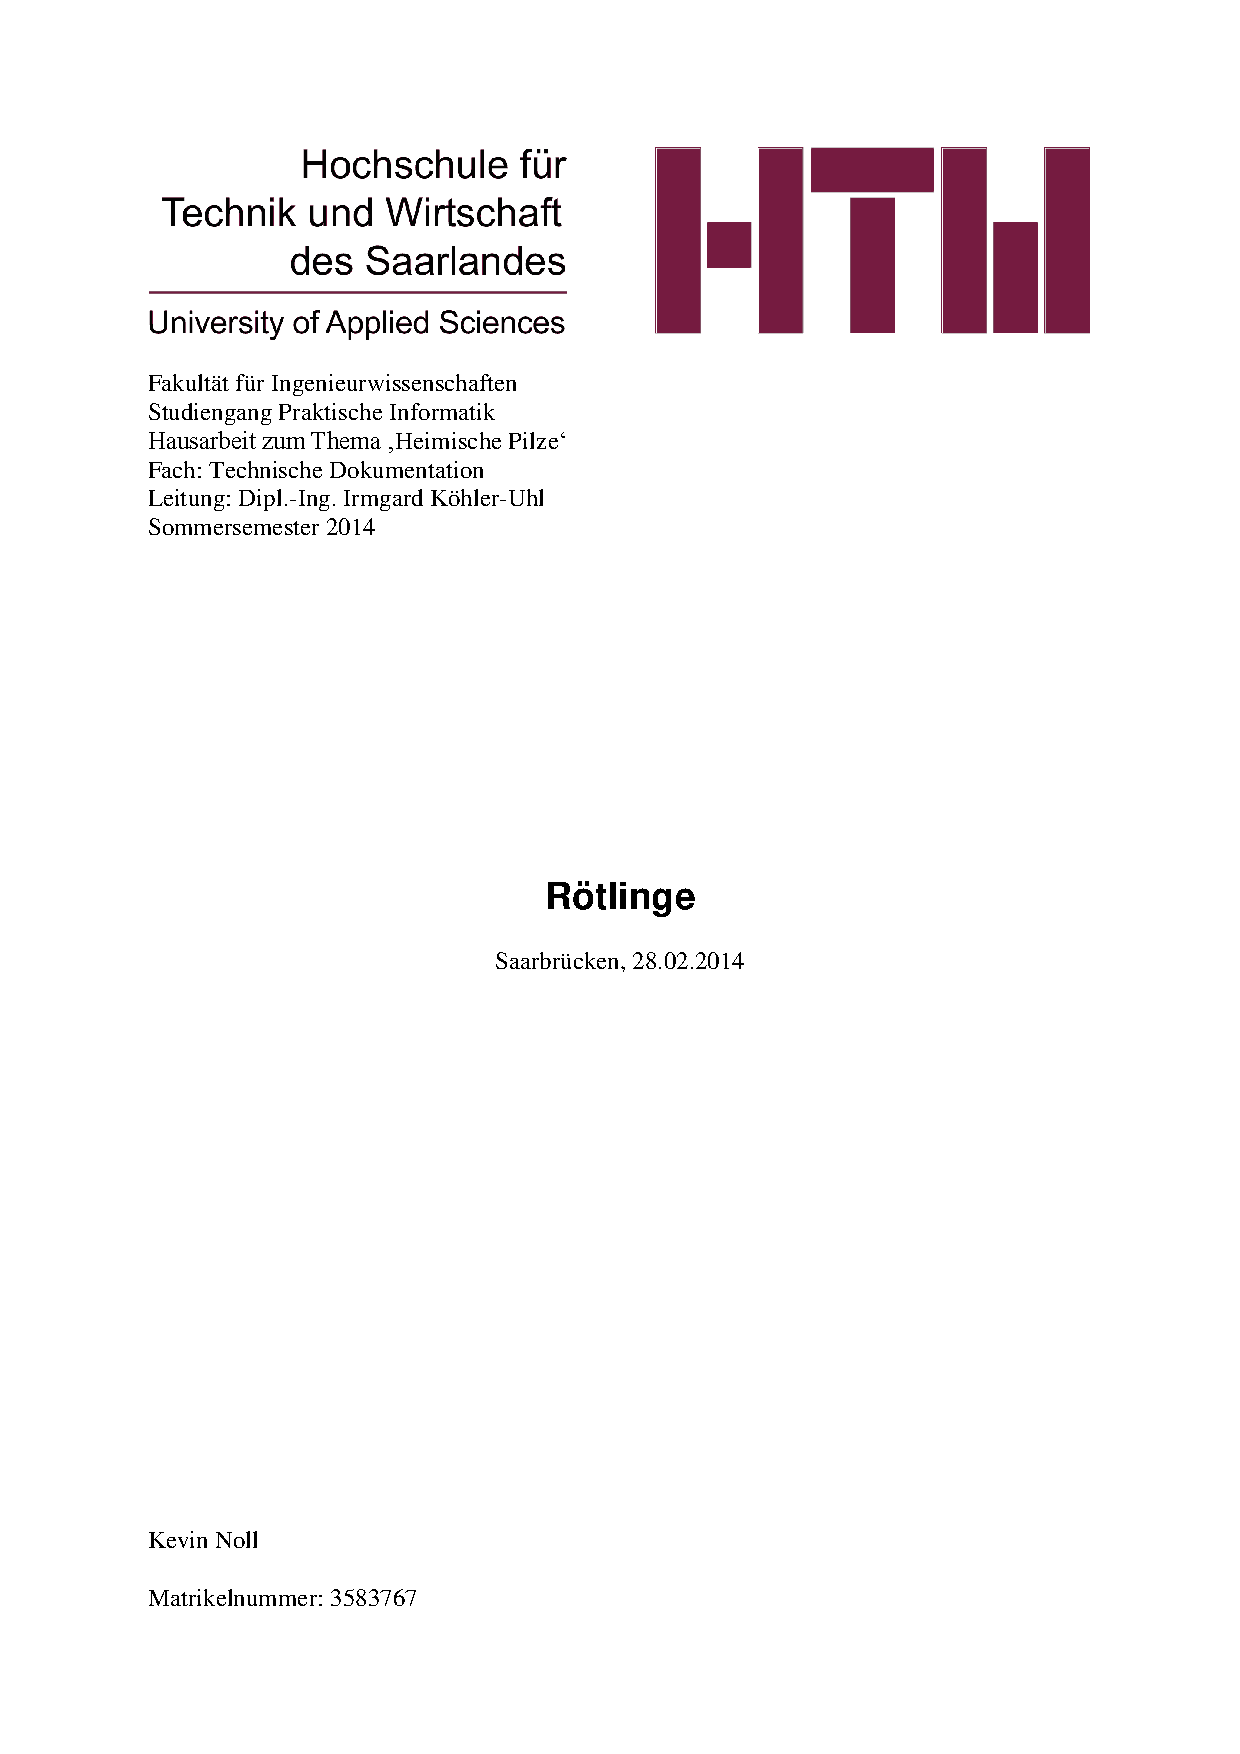
\includepdf[]{deckblatt.pdf}

%\author{Kevin Noll}
%\subject{Pilze und so}
%\title{Roetlinge, yo}
%\publishers{htwsaar}
%\maketitle
\tableofcontents
%\listoffigures
%\listoftables

\begin{abstract}
\begin{quote}%abstand rechts und links
Diese Arbeit befasst sich mit Pizlen und so nem kram. kein scheiss
\end{quote} 
\end{abstract}

\chapter{Vorwort}
Diese Ausarbeitung ist Bestandteil einer Reihe von Ausarbeitungen, die im Zuge der Vorlesung "'Technische Dokumentation"' entstanden sind. Der Kerngedanke bei der Anfertigung dieser Arbeit ist, zu erlernen, wie man mit fachbezogenen Texten umgeht -- von der Recherche über die Erstellung bis hin zur Anfertigung eines korrekten Literaturverzeichnisses. Unter dem Schirmthema \emph{Heimische Pilze} beschäftigt sich diese Ausarbeitung mit den Rötlingen (lat.: "'Entoloma"'). Es werden unter anderem Kenntnisse über die benötigte Bodenbeschaffenheit, die Beschreibung des Pilzes, die bei Pilzen so wichtigen Verwechslungsmöglichkeiten sowie die Zubereitung vermittelt.
\footnote{\autocite{entoloma}}
\chapter{Rötlinge}
\section{Allgemeines}
Rötlinge (lat.: "'Entoloma"') sind eine direkte Untergruppe -- auch Gattung genannt -- der Familie der Rötlingsverwandten (lat.: "'Entolomataceae"'). Wie alle Arten der Rötlingsverwandten besitzen die Rötlinge rosa- bis braunfarbenes Sporenpulver. Die Sporen der Rötlinge sind dabei im Gegensatz zu vielen anderen Gattungen der Familie eckig, was jedoch nur unter einem Mikroskop ersichtlich ist. Weiterhin besitzen viele Arten der Rötlinge sogenannte Zystiden. 
\section{Bodenbeschaffenheit}
\section{Beschreibung der Pilze}
\section{Verwechslungsmoeglichkeiten}
\section{Inhaltsstoffe, Geniessbarkeit}
\section{Ernte, Haltbarkeit und richtige Lagerung}
\section{Verwendung und Zubereitung mit Rezept}

%sadfsdf
\printbibliography


\end{document}